%\documentclass[10pt,dvipsnames,svgnames]{beamer}
\documentclass[aspectratio=169, lualatex, handout, 10pt,dvipsnames,svgnames]{beamer} %
\makeatletter\def\input@path{{theme/}}\makeatother\usetheme{cipher}

\title{Computer Security: Introduction}
\author{Markulf Kohlweiss}
\subject{Introduction to Applied Cryptography covering cryptographic primitives, protocols, security goals, and real-world applications from basic concepts to advanced topics like TLS and zero-knowledge proofs.}
\keywords{cryptography, security, encryption, authentication, hash functions, TLS, protocols, provable security}
\institute{University of Edinburgh, School of Informatics}
\instituteimage{images/edu-white.png}
\date{\today}
\coversubtitle{INFR10067\\Fall 2025}
\coverpartname{Cryptography}
\covertopicname{Cryptographic hash functions and MACs}
\coverwebsite{}

\mode<presentation>
{
  \usetheme{default}
  \usecolortheme{default}
  \usefonttheme{default}
  \setbeamertemplate{navigation symbols}{}
  \setbeamertemplate{caption}[empty]
  \setbeamertemplate{footline}[frame number]
}

\iffalse
\setbeamertemplate{blocks}[rounded][shadow=true]
\setbeamercolor{block title}{fg=black, bg=Grey!50}
\setbeamercolor{block body}{fg=black, bg=Grey!25}
\setbeamercolor{block title alerted}{fg=black, bg=Red!20}
\setbeamercolor{block body alerted}{fg=black, bg=Red!15}
\setbeamercolor{block title example}{fg=black, bg=SeaGreen!20}
\setbeamercolor{block body example}{fg=black, bg=Green!15}
\fi

\usepackage[english]{babel}
\usepackage[utf8x]{inputenc}

\usepackage[lambda,advantage,operators,sets,adversary,landau,probability,notions,logic,ff,mm,primitives,events,complexity,asymptotics,keys]{cryptocode}

\usepackage{graphicx}
\usepackage{tikz}
\usetikzlibrary{arrows.meta}
\usetikzlibrary{shapes.geometric}
\pgfdeclarelayer{background}
\pgfsetlayers{background,main}



\usepackage{scrextend}
\usepackage{eurosym}

\usepackage{fancybox}

\usepackage{pgfpages}

\usepackage{caption}
\usepackage{subcaption}

\usepackage{mdframed}
\usepackage{xspace}
\newcommand\Fontvi{\fontsize{5}{5.2}\selectfont}
\definecolor{ao}{rgb}{0.0, 0.6, 0.0}
\definecolor{bleu}{rgb}{0.2,0.2,0.7}

\newcommand{\Inred}[1]{\textcolor{BrickRed}{#1}}
\newcommand{\Inblue}[1]{\textcolor{bleu}{#1}}
\newcommand{\Ingreen}[1]{\textcolor{SeaGreen}{#1}}

\newcommand{\V}[1]{\texttt{V\textsubscript{{#1}}}\xspace}
\newcommand{\Vs}[1]{$\texttt{V}'_\texttt{{#1}}$\xspace}
\newcommand{\BB}{\texttt{BB}\xspace}
\newcommand{\EA}{\texttt{EA}\xspace}
\newcommand{\A}{\adv\xspace}
\newcommand{\F}[1]{$\mathcal{F}_\textsc{{#1}}$\xspace}
\renewcommand{\S}{\sdv\xspace}
\newcommand{\E}{$\mathcal{E}$\xspace}
\renewcommand{\P}{$P$\xspace}
\newcommand{\D}{\ddv\xspace}

\newcommand{\Pt}[2]{$\Pi^{{#2}}_{\textsc{{#1}}}$\xspace}

\newcommand{\Enc}{\texttt{Enc}}
\newcommand{\CheckShares}{\texttt{Check}}

\newcommand{\ASetup}{\texttt{ASetup}}
\newcommand{\AEval}{\texttt{AEval}}
\newcommand{\AWit}{\texttt{AWit}}
\newcommand{\AVer}{\texttt{AVer}}

\newcommand{\CSetup}{\texttt{CSetup}}
\newcommand{\CCommit}{\texttt{CCommit}}
\newcommand{\COpen}{\texttt{COpen}}

\newcommand{\SGen}{\texttt{SGen}}
\newcommand{\SSign}{\texttt{SSign}}
\newcommand{\SVer}{\texttt{SVer}}

\newcommand{\SoKSetup}{\texttt{SoKSetup}}
\newcommand{\SoKSign}{\texttt{SoKSign}}
\newcommand{\SoKVer}{\texttt{SoKVer}}

\newcommand{\TLEnc}{\texttt{TLEnc}}
\newcommand{\TLDec}{\texttt{TLDec}}

\newcommand{\frameindent}{\hspace*{\baselineskip}}

\colorlet{gris}{black!50!white}
\def\engris#1{\textcolor{gris}{#1}}

\colorlet{jaune}{yellow!90!black}
\def\enjaune#1{\textcolor{jaune!70!black}{#1}}

\colorlet{vert}{green!45!black}
\def\envert#1{\textcolor{vert}{#1}}

\colorlet{bleu}{blue!70!black}
\def\enbleu#1{\textcolor{bleu}{#1}}

\colorlet{rouge}{red!75!black}
\def\enrouge#1{\textcolor{rouge}{#1}}

\newcommand{\rouge}{\only{\color{rouge}}}

\xdefinecolor{violet}{rgb}{.5,0,.7}
\def\enviolet#1{\textcolor{violet}{#1}}

\xdefinecolor{violetft}{rgb}{0.199,0., 0.398}
\def\envioletft#1{\textcolor{violetft}{#1}}

\xdefinecolor{monbleu}{rgb}{0,.2,.54}
\newcommand{\monbleu}{\only{\color{monbleu}}}



\newcommand{\Ccal}{\mathcal{C}}
\newcommand{\Kcal}{\mathcal{K}}
\newcommand{\Mcal}{\mathcal{M}}
\newcommand{\Tcal}{\mathcal{T}}
\newcommand{\Xcal}{\mathcal{X}}


\title{Cryptography: cryptographic hash functions and MACs}

\author{Markulf Kohlweiss\\
  School of Informatics \\
  University of Edinburgh}



\date{}

\begin{document}

\begin{frame}
  \maketitle
\end{frame}

\begin{frame}{Introduction}
  \note{
    \begin{itemize}
    \item We mentioned malleability. 
    \item We will see that maleability might interfere with integrity and authenticity.
    \item Even though the data is encrypted.
    \end{itemize}
  }


  Encryption $\Rightarrow$ confidentiality against eavesdropping
  \bigskip{}
  \bigskip{}
  \pause

  What about authenticity and integrity against an active attacker?

  $\longrightarrow$ cryptographic hash functions and Message authentication codes

  $\longrightarrow$ this lecture


\end{frame}

\begin{frame}{One-way functions (OWFs)}

  A OWF is a function that is easy to compute but hard to invert:

  \begin{definition}[One-way]
    A function $f$ is a one-way function if for all $y$ there is no efficient algorithm which can compute $x$ such that $f(x)=y$
  \end{definition}
  \pause
  \bigskip{}


  \color{vert}

  Constant functions ARE NOT OWFs
  
  \quad any $x$ is such that $f(x)=c$
  \bigskip{} 
  \pause

  The successor function in $\mathbb N$ IS NOT a OWF

  \quad given $succ(n)$ it is easy to retrieve $n=succ(n)-1$
  \bigskip{} 
  \pause

  Multiplication of large primes IS a OWF:

  \quad integer factorisation is a hard problem - given $p\times q$ (where $p$ 

  \quad and $q$ are primes) it is hard to retrieve $p$ and $q$
  \color{black}

\end{frame}

\begin{frame}

  \frametitle{Collision-resistant functions (CRFs)}

  A function is a CRF if it is hard to find two messages that get mapped to the same value threw this function

  \begin{definition}[Collision resistance]
    A function $f$ is collision resistant if there is no efficient algorithm that can find two messages $m_1$ and $m_2$ such that $f(m_1) = f(m_2)$
  \end{definition}
  \bigskip{}
  \pause

  \color{vert}

  Constant functions ARE NOT CRFs
  
  \quad for all $m_1$ and $m_2$, $f(m_1) = f(m_2)$
  \bigskip{}
  \pause

  The successor function in $\mathbb N$ IS a CRF

  \quad the predecessor of a positive integer is unique
  \bigskip{} 
  \pause

  Multiplication of large primes IS a CRF:
    
  \quad every positive integer has a unique prime factorisation
  \color{black}


\end{frame}

\begin{frame}

  \frametitle{Cryptographic hash functions}

  \note{
    \begin{itemize}
    \item A cryptographic hash function h maps inputs x of arbitrary bit length to outputs h(x) of a fixed bit length n. This is known as the compression function.
    \end{itemize}
  }
  A cryptographic hash function takes messages of arbitrary length and returns a fixed-size bit string such that any change to the data will (with very high probability) change the corresponding hash value.

  \begin{definition}[Cryptographic hash function]
    A cryptographic hash function $H:\ \Mcal \rightarrow \Tcal$ is a function that satisfies the following 4 properties:
    \begin{itemize}
    \item $|\Mcal| >> |\Tcal|$
    \item it is easy to compute the hash value for any given message 
    \item it is hard to retrieve a message from it hashed value (OWF)
    \item it is hard to find two different messages with the same hash value (CRF)
    \end{itemize}
  \end{definition}
  \medskip{}
  
  \envert{Examples: MD4, MD5, SHA-1, RIPEMD160, SHA-256, SHA-512, SHA-3\dots}\medskip

  \enrouge{$\rightsquigarrow$In new projects use SHA-256 or SHA-512 or SHA-3}

  

  \note{
    \begin{itemize}
    \item Practical hash functions: MD4, MD5, MD4, MD5, RIPEMD160, SHA-1, SHA-256, SHA-512, Whirlpool, \dots
    \item MD4, MD5, considered not secure, SHA-1 neither
    \item Functions widely believed to perform in practice like a cryptographic hash function
    \item No mathematical proof that they satisfy CR or OW
    \item No significant attacks known
    \item Standardised by NIST
    \end{itemize}
  }
  
\end{frame}

\begin{frame}

  \frametitle{Cryptographic hash functions: applications}

  \note{
    \begin{itemize}
    \item File integrity - Alice stores her files on a cloud server. She later retrieves the files. How can she make sure the files were not corrupted. She wants something more efficient than keeping a copy of all her files.\medskip
    \item Password authentication - How to authenticate users without storing passwords? We want to avoid a server breach to leak passwords. We want to defend against password guessing atacks.
    \end{itemize}
  }

  \begin{itemize}
  \item {\bf Commitments -} Allow a participant to commit to a value $v$ by publishing the hash $H(v)$ of this value, but revealing $v$ only later. \envert{Ex: electronic voting protocols, digital signatures, \dots}
    \medskip{}
    \pause

  \item {\bf File integrity -} Hashes are sometimes posted along with files on ``read-only'' spaces to allow verification of integrity of the files. \envert{Ex: SHA-256 is used to authenticate Debian GNU/Linux software packages}
    \medskip{}
    \pause

  \item {\bf Password verification -} Instead of storing passwords in cleartext, only the hash digest of each password is stored. To authenticate a user, the password presented by the user is hashed and compared with the stored hash.
    \medskip{}
    \pause

    
  \item {\bf Key derivation -} Derive new keys or passwords from a single, secure key or password.
    \medskip{}
    \pause

  \item {\bf Building block of other crypto primitives -} Used to build MACs, block ciphers, PRG, \dots
  \end{itemize}

\end{frame}

\begin{frame}{Collisions are unavoidable}

  \begin{center}
    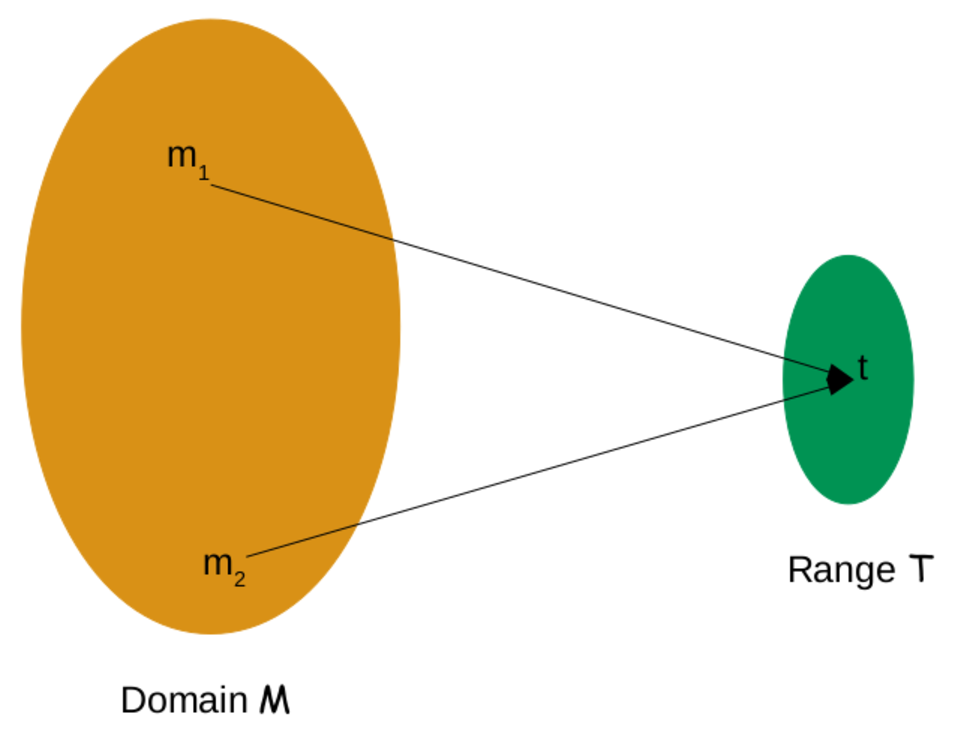
\includegraphics[scale=0.5]{Images/Collisions.pdf}
  \end{center}

  The domain being much larger than the range, collisions necessarily exist
  
\end{frame}

\begin{frame}

  \frametitle{The birthday attack - attack on all schemes}
  \pause

  \note{
    \begin{itemize}
    \item The chief way that cryptographic hash function are attacked is by compromising their collision resistance. 
    \item This can be done by using a brute force technique known as a birthday attack.
    \item Suppose that a cryptographic hash function, $H$, has a $n$-bit output. We have that the number of possible hash values is $2^n$. We might at first thing that an attacker, Eve, needs to generate a number of inputs proportional to $2^n$ before she finds a collision, but this is not the case.
    \item In the birthday attack, Eve computes a large number of random messages and computes the cryptographic hash value of each one hoping to find two messages with the same hash value. 
    \item \enrouge{The probability of finding a collision with in this $2^{n/2}$ messages is greater than $50\%$}
    \item For an $n$-bit hash $y$, the expected number of tries before an $x$ with $h(x)=y$ is found is $2^{n}-1$. 
    \item If you are looking for arbitrary collisions, as set of about $2^{n/2}$ inputs is likely to contain a pair causing a collision. 
    \end{itemize}
  }

  \begin{theorem}
    Let $H:\ \Mcal\rightarrow \{0, 1\}^n$ be a cryptographic hash
    function ($|\Mcal| >> 2^n$)

    Generic algorithm to find a collision in time $O(2^{n/2})$ hashes:
    \begin{enumerate}
    \item Choose $2^{n/2}$ random messages in $\Mcal$: $m_1, \dots,
      m_{2^{n/2}}$
    \item For $i=1, \dots, 2^{n/2}$ compute $t_i = H(m_i)$
    \item If there exists a collision ($\exists i, j.\ t_i= t_j$)
    
      then return $(m_i, m_j)$

      else go back to 1
    \end{enumerate}
  \end{theorem}

  \underline{Birthday paradox} Let $r_1, \dots, r_\ell\in\{1, \dots, N\}$ be independent variables. For $\ell=1.2\times \sqrt N$, $Pr(\exists i\not=j.\ r_i=r_j)\ge \frac 1 2$\bigskip

  \quad $\Rightarrow$ the expected number of iteration is 2 

  \quad $\Rightarrow$ running time $O(2^{n/2})$ 
  \bigskip{}

 \enrouge{$\Rightarrow$ Cryptographic function used in new projects should have an output size $n\ge 256$!}

\end{frame}

\begin{frame}

  \frametitle{The Merkle-Damgard construction}
\vspace{-0.7cm}
  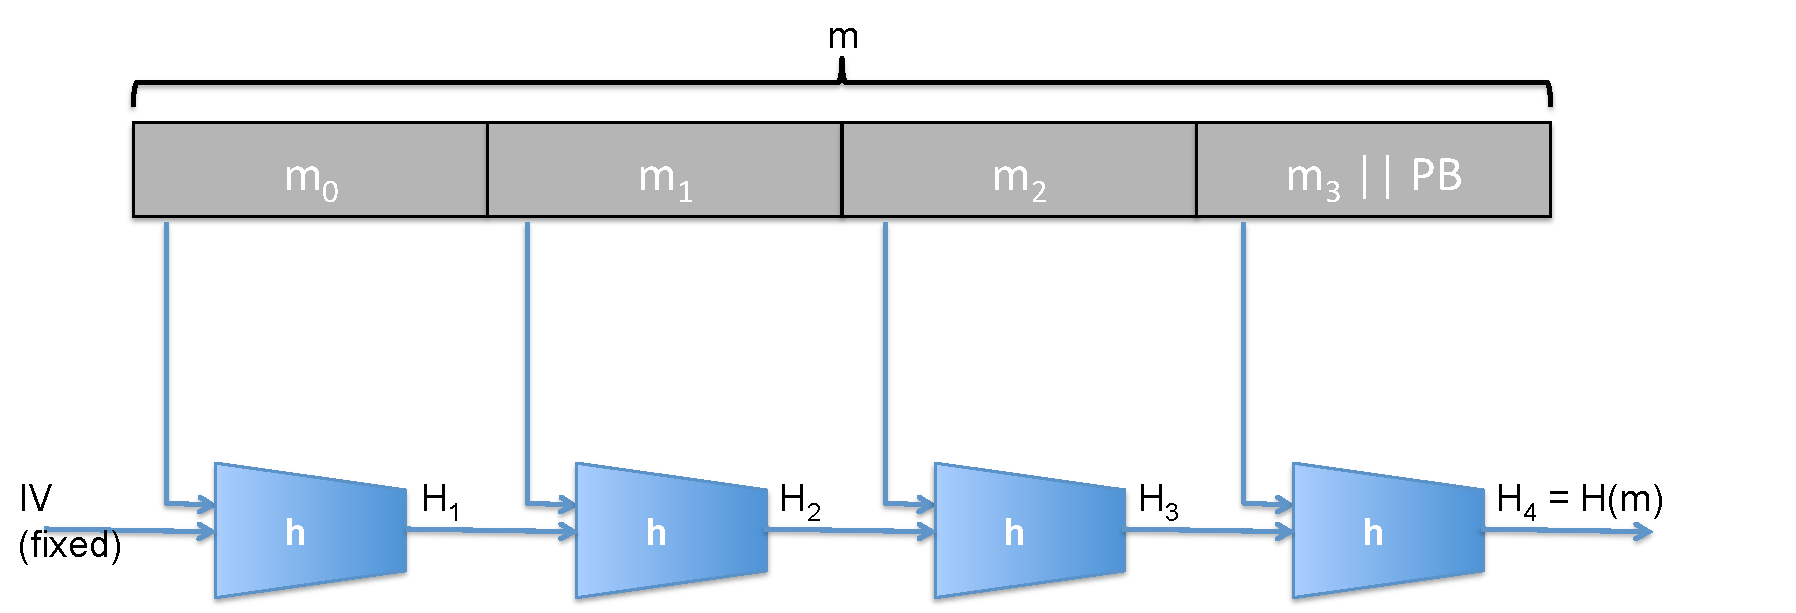
\includegraphics[scale=0.4]{Images/MerkleDamgard.pdf}

  \begin{itemize}
  \item Compression function: $h:\ \Tcal \times \Xcal \rightarrow \Tcal$
  \item PB: $1000 \dots 0 || \mathsf{mes\text{-}len}$ (add extra block if needed) \\ \enrouge{(different variants!)}
  \end{itemize}
  \medskip{}
  \begin{theorem}
    Let $H$ be built using the MD construction to the compression
    function $h$. If $H$ admits a collision, so does $h$.
  \end{theorem}
  \medskip{}

  \envert{Example of MD constructions: MD5, SHA-1, SHA-2, \dots}

\end{frame}

\begin{frame}

  \frametitle{Compression functions from block ciphers}

  Let $E:\ \Kcal \times \{0, 1\}^n \rightarrow \{0, 1\}^n$ be a block cipher
  \bigskip

  \begin{figure}[c]
    \centering
    \begin{tabular}{ccc}
      \hspace{-0.8cm}\onslide<2->{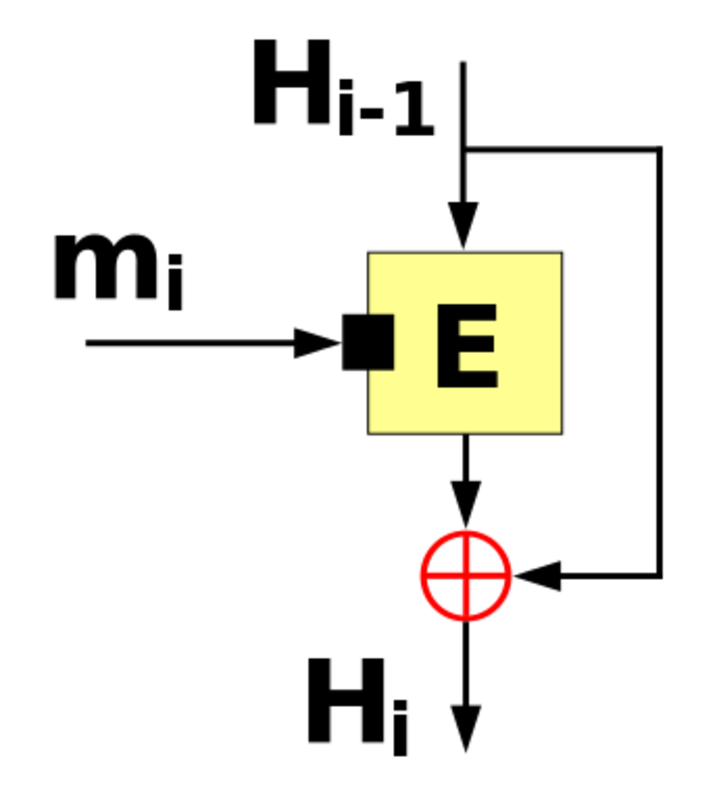
\includegraphics[scale=0.25]{Images/Davies-Meyer_hash.pdf}} & \hspace{1cm} & \onslide<3->{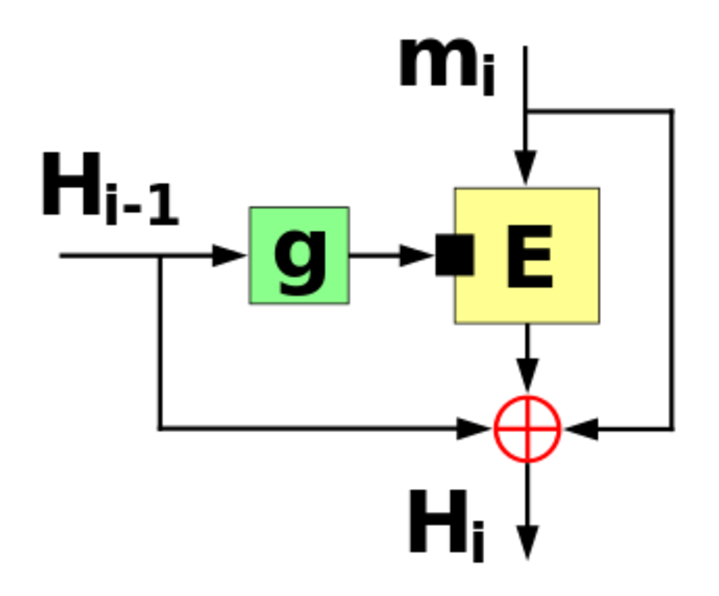
\includegraphics[scale=0.25]{Images/Miyaguchi-Preneel_hash.pdf}} \\
      \hspace{-0.8cm}\onslide<2->{Davies-Meyer} & \hspace{1cm} & \onslide<3->{Miyaguchi-Preneel}
    \end{tabular}
    
    \caption*{\onslide<2->{\engris{Source: \url{https://en.wikipedia.org/wiki/One-way_compression_function}}}}
  \end{figure}
\end{frame}

\begin{frame}
  \frametitle{Example of cryptographic hash function: SHA-256}

  \begin{itemize}
  \item Structure: Merkle-Damgard
  \item Compression function: Davies-Meyer
  \item Bloc cipher: SHACAL-2
    \begin{center}
      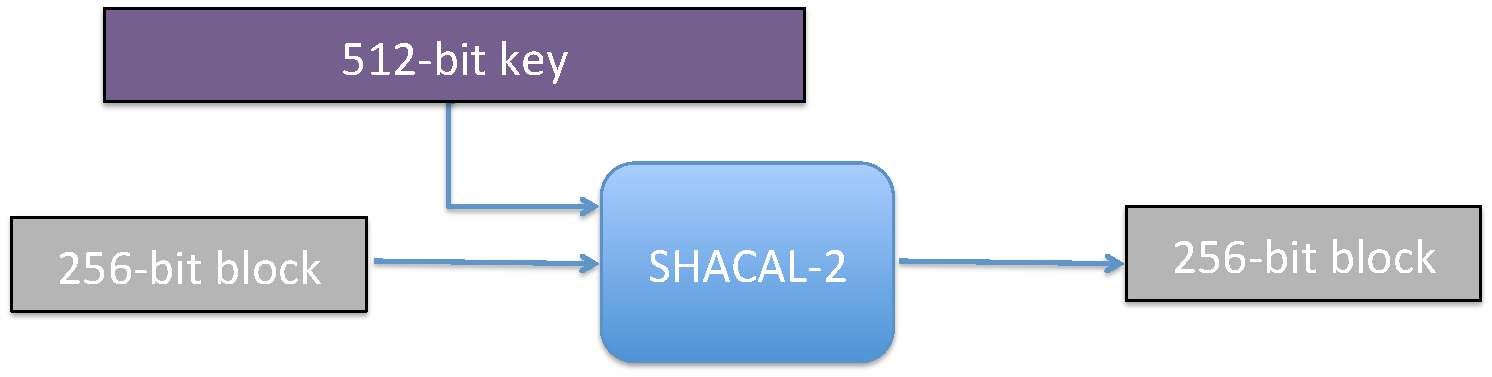
\includegraphics[scale=0.4]{Images/SHA-256.pdf}
    \end{center}
  \end{itemize}
\end{frame}



\covertopicname{Message Authentication Codes (MACs)}
\author{}
\date{}

\begin{frame}
  \maketitle
\end{frame}

\begin{frame}{\onslide<3->{Encryption is not always enough}}

  \[
    \begin{array}[c]{ccc}
      \begin{array}[c]{c}
        \hspace{-0.75cm}\includegraphics<1->[scale=0.2]{Images/su-mei-tse.pdf}
      \end{array}
      &
      \begin{array}[c]{c}
        \hspace{-0.5cm}\xrightarrow[]{e=E(K_E, \text{Transfer 100 } \footnotesize{\geneuro{}} \text{ on Bob's account})}
      \end{array}
      &
      \begin{array}[c]{c}
        \hspace{-0.5cm}\includegraphics<1->[scale=0.3]{Images/RBS-logo.pdf}
      \end{array}
    \end{array}
  \]
  \pause
  \begin{center}
    \enrouge{What if the encryption scheme $E$ is the OTP - $e=K_E \oplus \text{Transfer 100 } \footnotesize{\geneuro{}} \text{ on Bob's account}$?}
  \end{center}
  \pause
  \bigskip{}
  
  \[\hspace{-0.75cm}
    \begin{array}[c]{ccccc}
      \begin{array}[c]{c}
        \phantom{\includegraphics<1-2>[scale=0.2]{Images/su-mei-tse.pdf}}
        \includegraphics<3->[scale=0.2]{Images/su-mei-tse.pdf}
      \end{array}
      & 
      \begin{array}[c]{c}
        \xrightarrow[]{e}
      \end{array}
      &
      \begin{array}[c]{c}
        \hspace{-0.75cm}
        \phantom{\includegraphics<1-2>[scale=0.2]{Images/intruder.pdf}}
        \includegraphics<3->[scale=0.2]{Images/intruder.pdf}
      \end{array}
      &
        \begin{array}[c]{c}
          \xrightarrow[\enrouge{=E(K_E, \text{Transfer 100 } \footnotesize{\geneuro{}} \text{ on Eve's account})}]{\enrouge{e\oplus \text{0\dots0Bob0\dots0}\oplus \text{0\dots0Eve0\dots0}}}
        \end{array}
      &
      \begin{array}[c]{c}
        \hspace{-1.35cm}
        \phantom{\includegraphics<1-2>[scale=0.3]{Images/RBS-logo.pdf}}
        \includegraphics<3->[scale=0.3]{Images/RBS-logo.pdf}
      \end{array}
    \end{array}
    \]
  
\end{frame}

\begin{frame}

  \frametitle{Goal: message integrity}
\vspace{-0.75cm}
  \note{
  \begin{tabular}{l}
    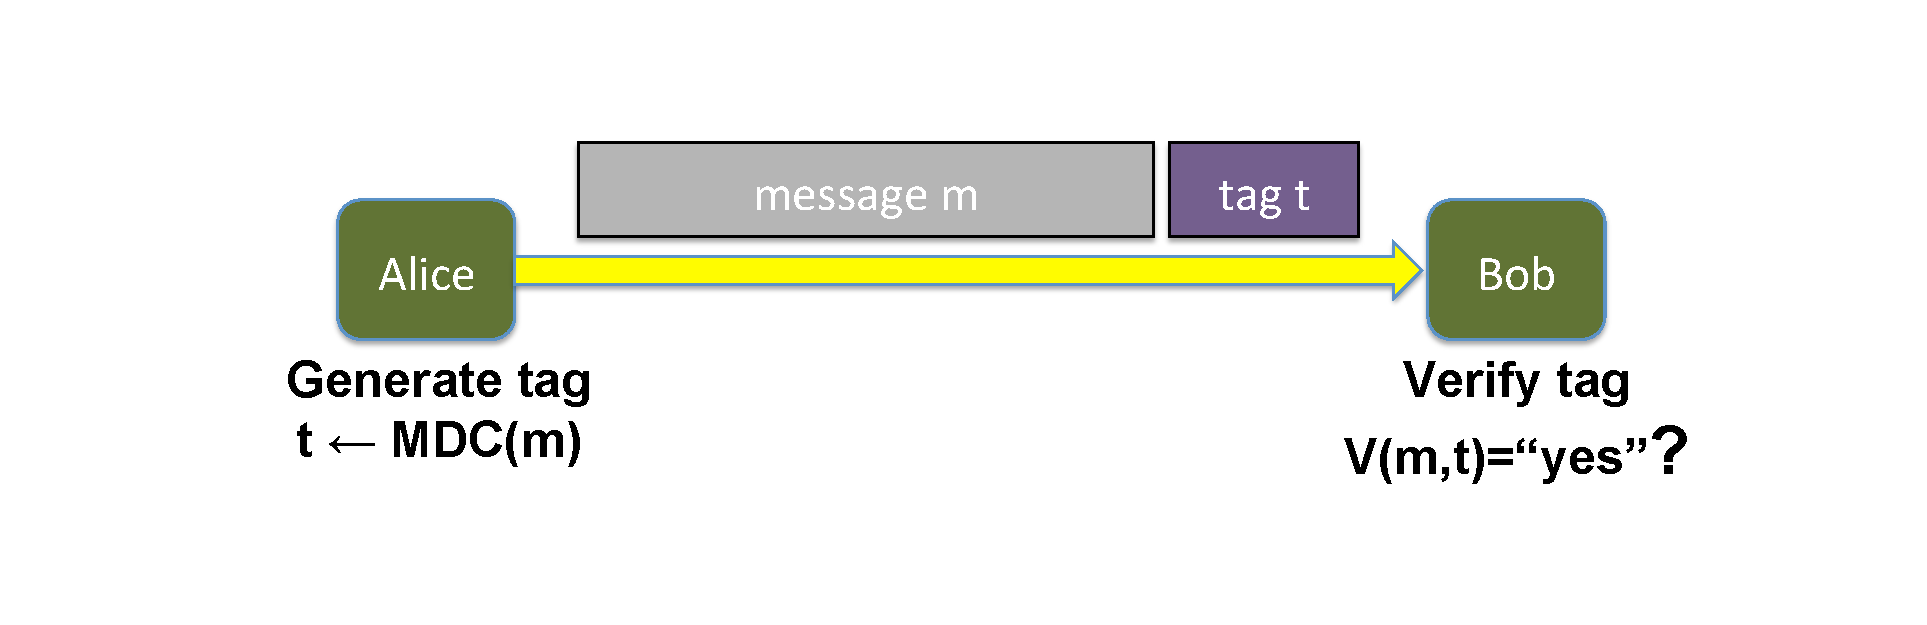
\includegraphics[scale=0.4]{Images/integrity2.pdf}
  \end{tabular}}
  
  \begin{tabular}{l}
    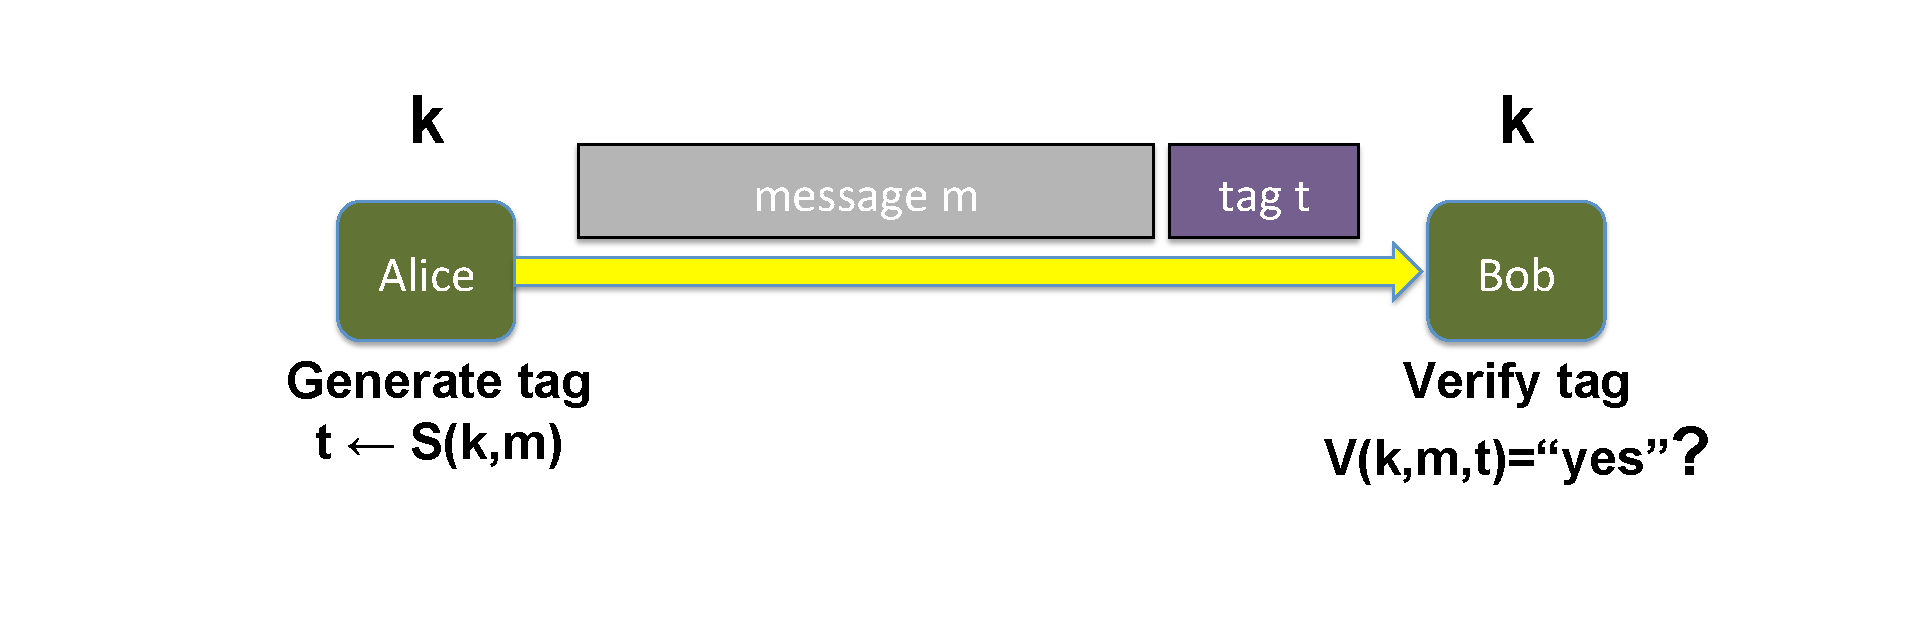
\includegraphics[scale=0.4]{Images/integrity1.pdf}
  \end{tabular}
  \pause

\vspace{-0.3cm}
  A MAC is a pair of algorithms $(S, V)$ defined over $(\Kcal, \Mcal, \Tcal)$:
  \begin{itemize}
  \item $S: \Kcal \times \Mcal\rightarrow \Tcal$
  \item $V: \Kcal \times \Mcal \times \Tcal\rightarrow \{\top,\bot\}$
  \item Consistency: $V(k, m, S(k, m)) = T$
  \end{itemize}
  
  \begin{alertblock}{Unforgeability}
  It is hard to computer a valid pair $(m, S(k, m))$ without knowing $k$
  \end{alertblock}
\end{frame}

\begin{frame}

  \frametitle{File system protection}
\vspace{-0.5cm}
  \begin{itemize}
  \item At installation time
    \begin{center}
      \begin{tabular}{c}
        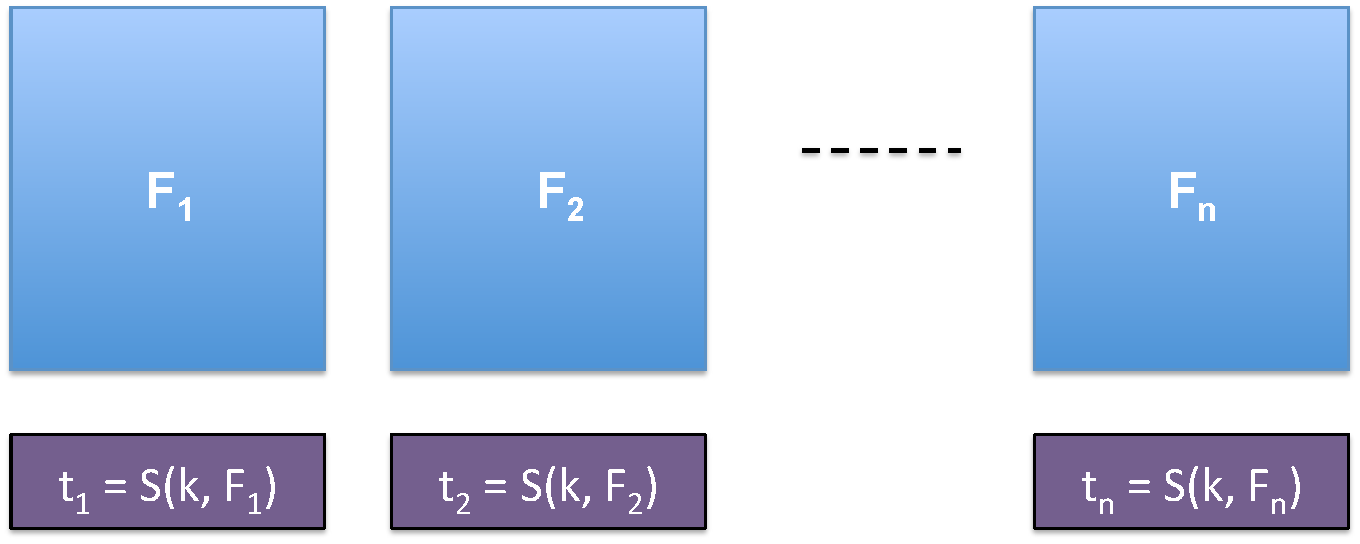
\includegraphics[scale=0.4]{Images/fileProtection.pdf} \\
        $k$ derived from user password
      \end{tabular}
    \end{center}
    \medskip{}
  \item To check for virus file tampering/alteration:
    \begin{itemize}
    \item reboot to clean OS
    \item supply password
    \item any file modification will be detected
    \end{itemize}
  \end{itemize}

\end{frame}

\begin{frame}
  \frametitle{Block ciphers and message integrity}
  \pause

  Let $(E, D)$ be a block cipher. We build a MAC $(S, V)$ using $(E, D)$ as follows:
  \begin{itemize}
  \item $S(k, m) = E(k, m)$
  \item $V(k, m, t) =
    \begin{array}[t]{l}
      \mathsf{if}\ m = D(k, t) \\
      \mathsf{then\ return}\ \top \\
      \mathsf{else\ return}\ \bot
    \end{array}
    $
  \end{itemize}
  \bigskip{}
  \pause

  {\bf But:} block ciphers can usually process only 128 or 256 bits
  \bigskip{}
  \pause

  {\bf Our goal now:} construct MACs for long messages

\end{frame}

\begin{frame}

  \frametitle{ECBC-MAC}
\vspace{-0.5cm}
  
  \begin{center}
    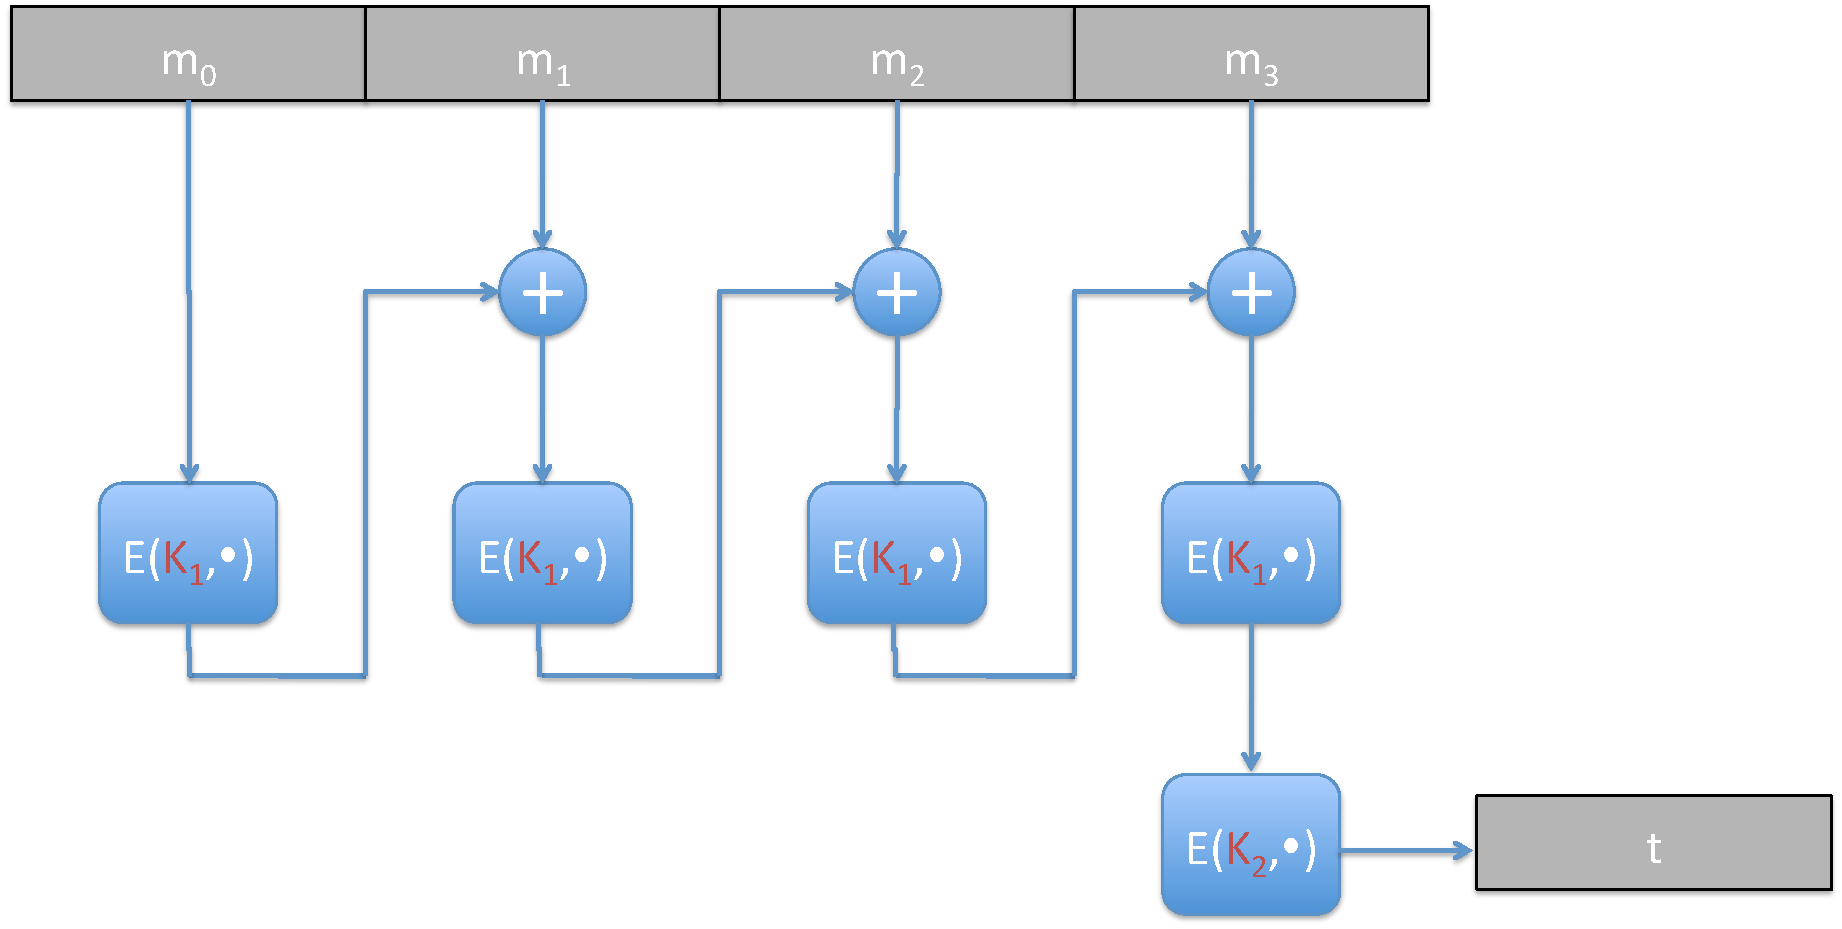
\includegraphics[scale=0.3]{Images/ECBC-MAC.pdf}
  \end{center}

  \begin{itemize}
  \item $E:\ \Kcal\times \{0, 1\}^n\rightarrow \{0, 1\}^n$ a block cipher
  \item $ECBC\text{-}MAC: \Kcal^2\times \{0, 1\}^*\rightarrow \{0, 1\}^n$
  \end{itemize}
  \enrouge{$\rightarrow$ the last encryption is crucial to avoid forgeries!!}

  \envert{Ex: 802.11i uses AES based ECBC-MAC}
\end{frame}

\begin{frame}

  \frametitle{PMAC}

  \vspace{-1.2cm}
  \begin{center}
    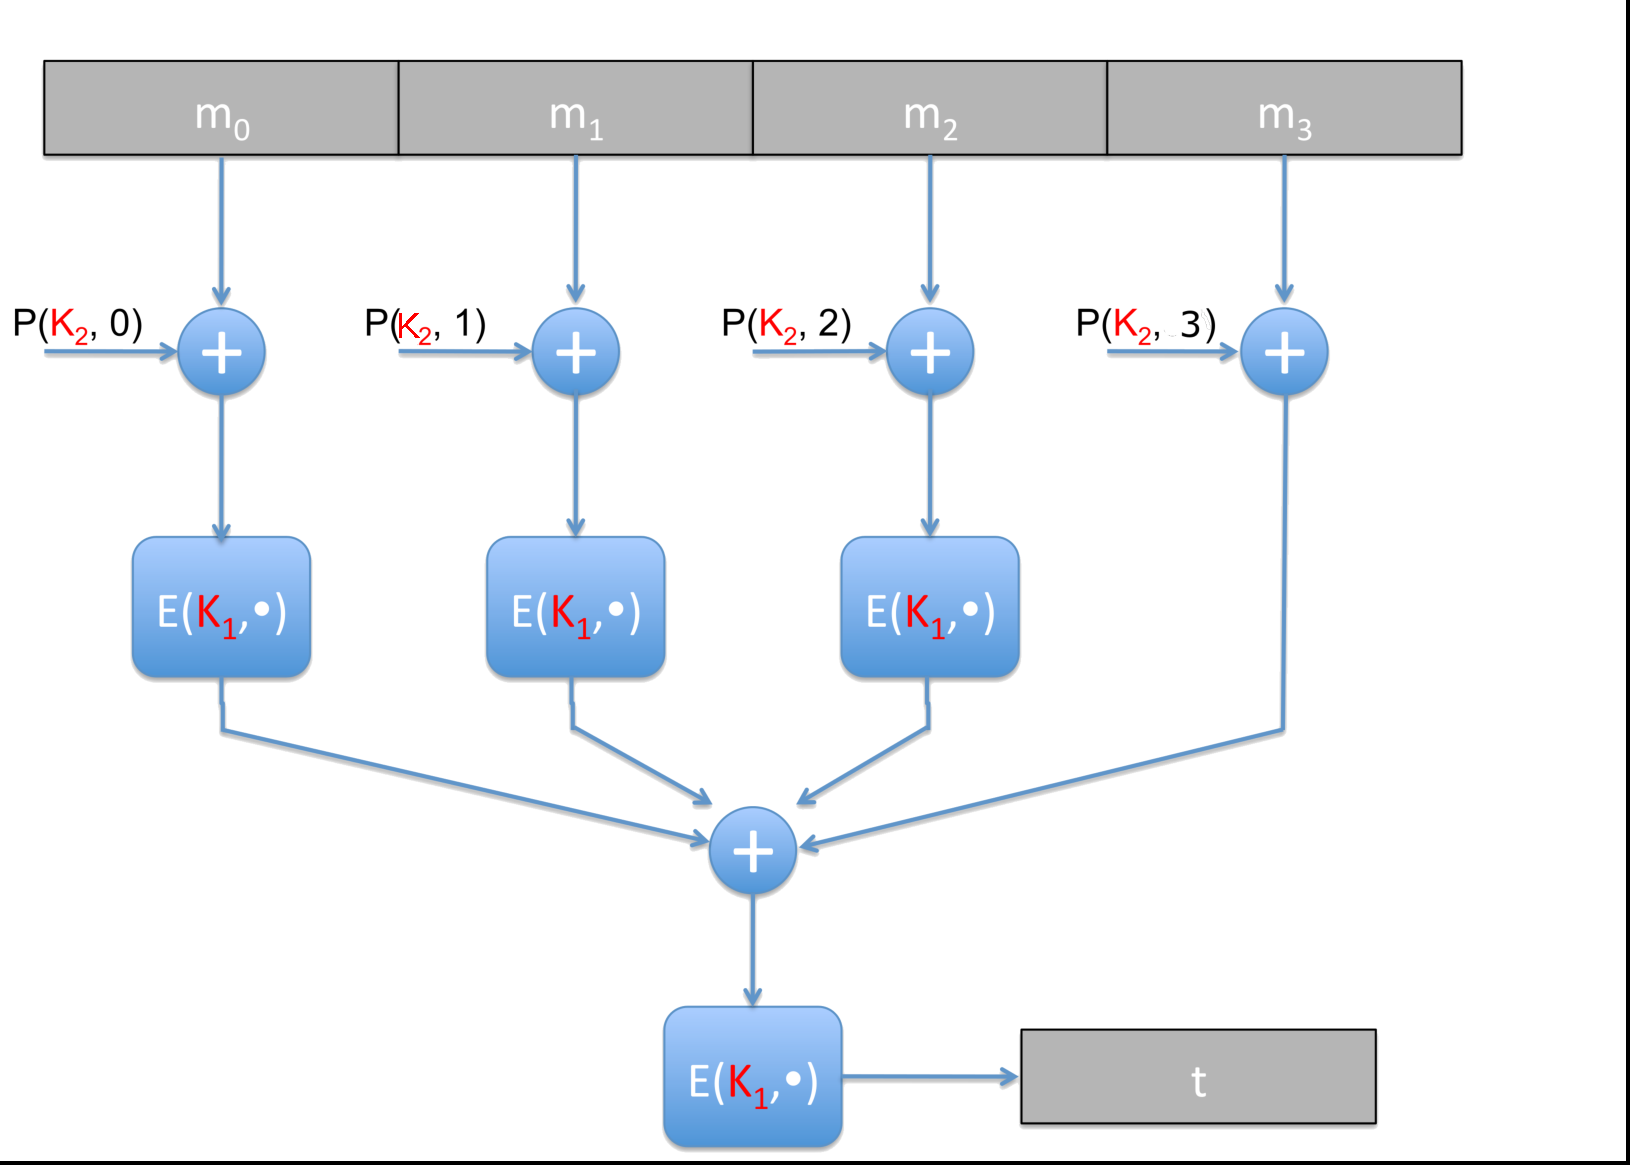
\includegraphics[scale=0.32]{Images/PMAC.pdf}
  \end{center}


  \begin{itemize}
  \item $E:\ \Kcal\times \{0, 1\}^n\rightarrow \{0, 1\}^n$ a block cipher
  \item $P:\ \Kcal\times \mathbb N\rightarrow \{0, 1\}^n$ an easy to compute function
  \item $PMAC: \Kcal^2\times \{0, 1\}^*\rightarrow \{0, 1\}^n$
  \end{itemize}
  \engris{See also: \url{https://www.youtube.com/watch?v=gZiBYDX9Fpo}}
\end{frame}

\begin{frame}

  \frametitle{HMAC}
\vspace{-0.4cm}
    MAC built from cryptographic hash functions
    \[
    HMAC(k, m) = H(k\oplus OP ||H(k\oplus IP||m))
    \]
    $IP, OP$: publicly known padding constants
    \bigskip{}
    
    \begin{center}
      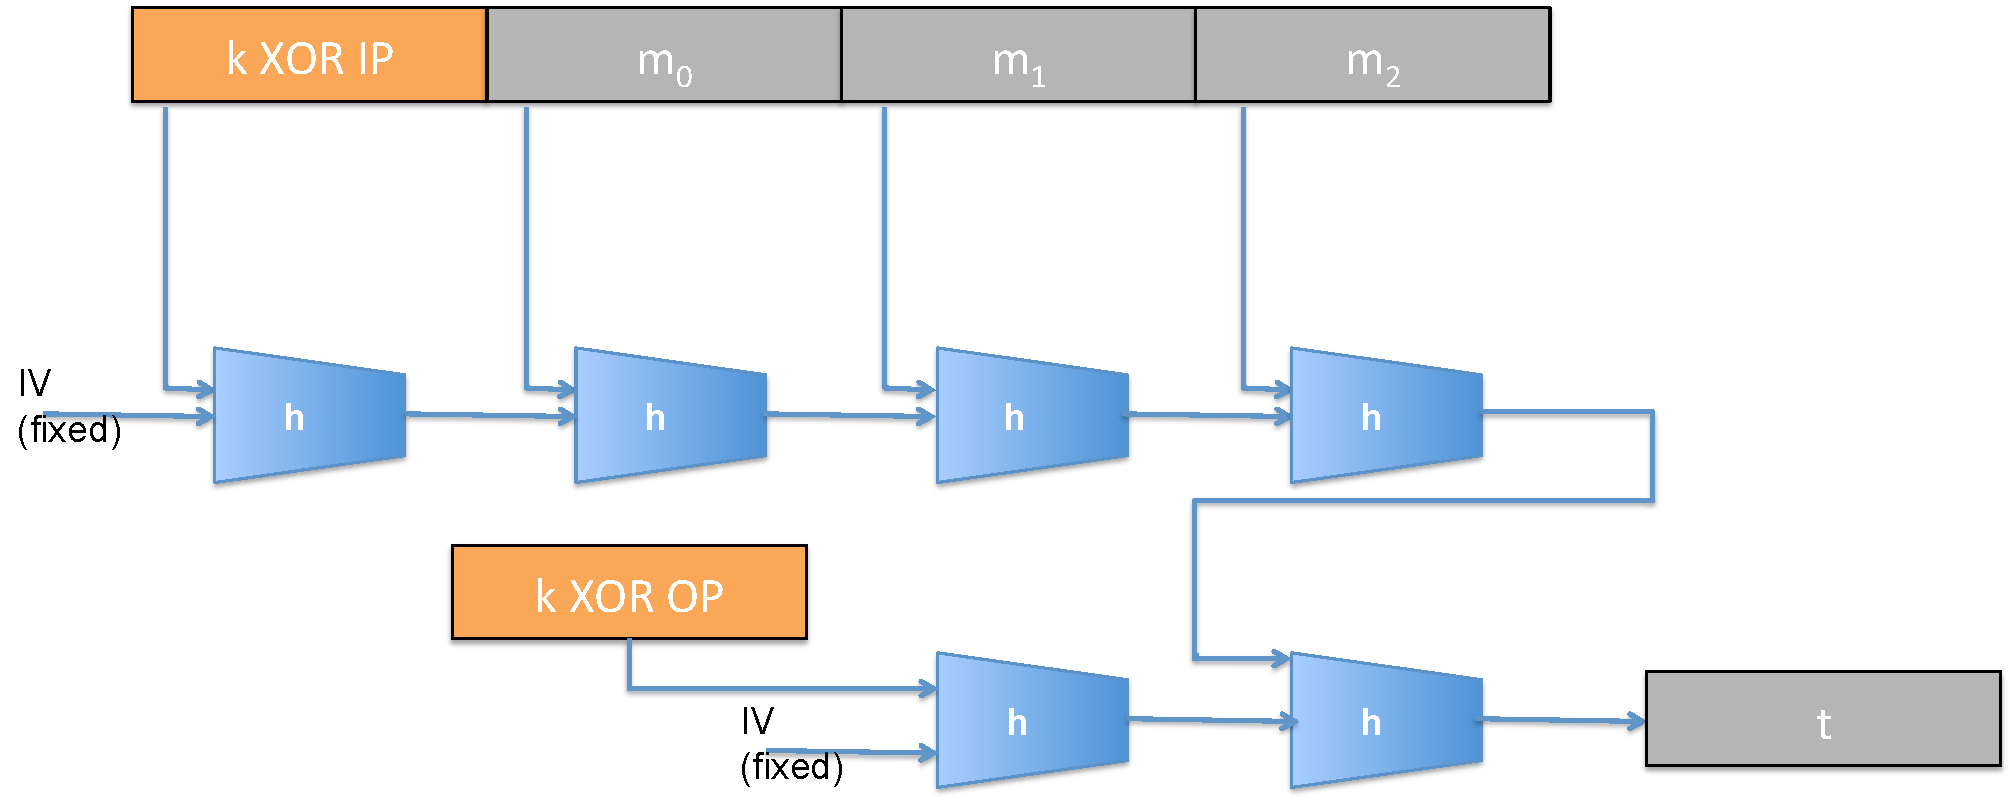
\includegraphics[scale=0.3]{Images/HMAC.pdf}
    \end{center}

    
  \envert{Ex: SSL, IPsec, SSH, \dots}

\end{frame}

\begin{frame}

  \frametitle{Naive MAC from Hashing}

  Simplest way to build a MAC from a hash function, prepend the key:
  \[
  MAC(k,m) = H(k \| m)
  \]

  This is not generally secure, but works for SHA3/Keccak as it prevents length extension attack. \\ \

\engris{Source: \url{https://keccak.team/keccak_strengths.html}} \\ \ \\ 

\engris{See also: \url{https://crypto.stackexchange.com/questions/1070/why-is-hk-mathbin-vert-x-not-a-secure-mac-construction}}
\end{frame}


\covertopicname{Authenticated encryption}

\begin{frame}
  \maketitle
\end{frame}


\begin{frame}
  \frametitle{Plain encryption is malleable}

  \begin{itemize}
  \item The decryption algorithm never fails
  \item Changing one bit of the $i^{th}$ block of the ciphertext
    \begin{itemize}
    \item CBC decryption: will affect last blocks after the $i^{th}$ of the plaintext
    \item ECB decryption: will only the $i^{th}$ block of the plaintext
    \item CTR decryption: will only affect one bit of the $i^{th}$ block of the plaintext
    \end{itemize}
    
  \end{itemize}
  \bigskip{}

  \begin{block}{}
    Decryption should fail if a ciphertext was not computed using the key
  \end{block}
  \begin{block}{Goal}
    Simultaneously provide data \enrouge{confidentiality}, \enrouge{integrity} and \enrouge{authenticity}
    
    \enrouge{$\rightsquigarrow$} decryption combined with integrity verification in one step
  \end{block}


\end{frame}

\begin{frame}
  \frametitle{Encrypt-then-MAC}

  \begin{enumerate}
  \item Always compute the MACs on the ciphertext, never on the plaintext
  \item Use two different keys, one for encryption ($K_E$) and one for the MAC ($K_M$)
  \end{enumerate}
  \bigskip{}

  \begin{block}
  \small
  \begin{columns}
    \begin{column}[c]{2in}
      \enrouge{Encryption}
      \begin{enumerate}
      \item $C\leftarrow E_{AES}(K_E, M)$
      \item $T\leftarrow HMAC$-$SHA(K_M, C)$
      \item return $C||T$
      \end{enumerate}
    \end{column}
    \begin{column}[c]{2in}
      \enrouge{Decryption}
      \begin{enumerate}
      \item if $T=HMAC$-$SHA(K_M, C)$
      \item then return $D_{AES}(K_E, C)$
      \item else return $\bot$
      \end{enumerate}
    \end{column}
  \end{columns}
\end{block}
  \bigskip{}
  \normalsize

  \enrouge{\bf Do not:}
  \begin{itemize}
  \item Encrypt-and-MAC: $E_{AES}(K_E, M) || HMAC$-$SHA(K_M, M)$
  \item MAC-then-Encrypt: $E_{AES}(K_E, M|| HMAC$-$SHA(K_M, M)) $
  \end{itemize}

\end{frame}

\begin{frame}{AES GCM}

  \begin{block}{Galois Counter Mode}
    Combines
    \begin{enumerate}
    \item \enrouge{Galois field} based One-time MAC for authentication
    \item \enrouge{AES} based Counter Mode for encryption
    \end{enumerate}
  \end{block}
  \bigskip{}

  \begin{itemize}
  \item \enrouge{Trick}: One-time MAC is encrypted too

    $\Rightarrow$ secure for many messages
    
  \item Widely adopted for its performance
    
  \item Many good implementations of this mode
  \end{itemize}
  
\end{frame}
\end{document}
